%!TEX program = xelatex
\documentclass[letterpaper,12pt]{exam}
\usepackage{../videoNotes}
\usepackage[dvipsnames]{xcolor}
\usepackage{soul}
\usepackage{tabulary}
\usepackage{fontspec}

\usepackage{draftwatermark}
\SetWatermarkText{Draft}
\SetWatermarkScale{1.5}
\SetWatermarkColor{red!20}

\newcommand{\unit}{Unit 09}
\pagestyle{headandfoot}
\firstpageheader{CSC 264 \semester\ \  \unit}{}{Name: $\rule{6cm}{0.15mm}$}
\runningheader{CSC 264 \semester}{\unit}{Page \thepage\ of \numpages}
\firstpagefooter{}{}{}
\runningfooter{}{}{}

\begin{document}

%\underconstruction

\par{\fontfamily{qzc}\selectfont\textbf{}}
\begin{questions}

\section*{\unit\_010 -- LEA (Part 1)}
\begin{samepage}
    \question What does LEA stand for?
    \vspace{5mm}
\end{samepage}
\par
\begin{samepage}
    \question How does the SYNTAX of the LEA instruction compare to the SYNTAX of the MOV instruction?
    \vspace{5mm}
\end{samepage}
\begin{samepage}
    \question How does the MEANING of the LEA instruction compare to the MEANING of the MOV instruction?
    \vspace{5mm}
\end{samepage}
\par
\begin{samepage}
    \question The following image is from the ddd debugger.  It shows the memory contents after lines 13 and 14 of the code were executed.  Why are the contents of r11 and r12 different?
   \begin{center}
    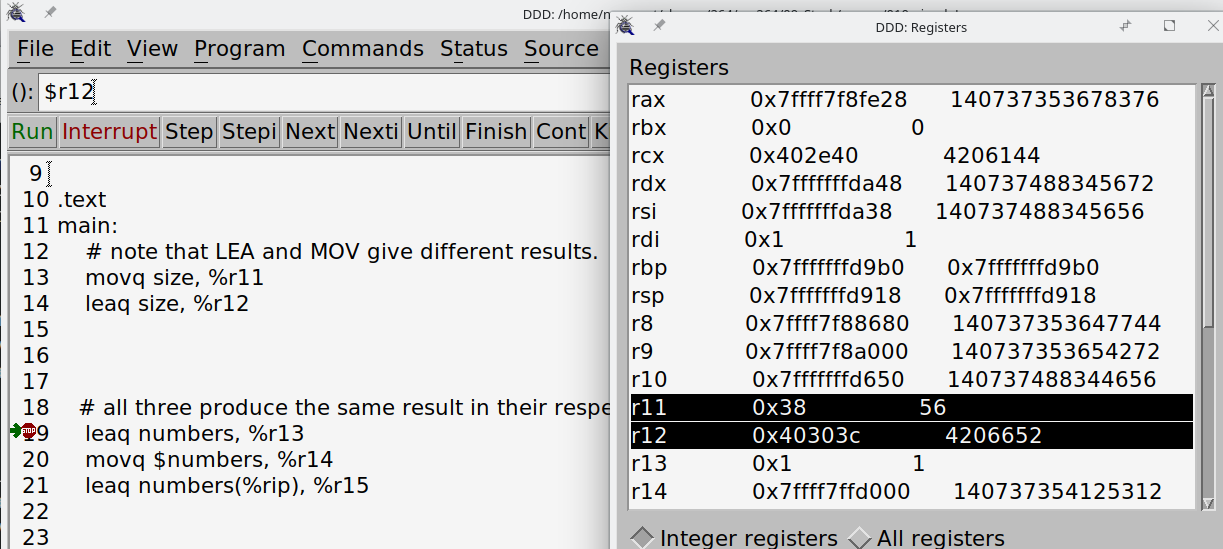
\includegraphics[width=\textwidth]{../../09_Stack/images/010_LeaVsMov.png}
   % \includegraphics{../images/unit09_010_LeaVsMov.png}
   \end{center}
   \vspace{5mm}
\end{samepage}
\par
 \section*{\unit\_010 -- LEA (Part 2)}
 \begin{samepage}
     \question Explain why using the "\$" in the statement  \texttt{\textbf{movq \$size, \%r11}} reduces the need for the \texttt{\textbf{lea}} instruction.
     \vspace{5mm}
 \end{samepage}
 \par
  
 \begin{samepage}
     \question In the GAS assember in 64-bit mode, which of the following statements is different than the others in their results?  Explain your answer.
     \begin{itemize}
             \item{texttt{movq size, \%r11}}
            \item {texttt{movq \$size, \%r11}}
            \item {texttt{leaq size, \%r11}}
           \end{itemize}
     \vspace{5mm}
 \end{samepage}
     \question In the GAS assember in 64-bit mode, which of the following statements is different than the others in their results?  Explain your answer.

 \begin{itemize}
             \item{texttt{movq size, \%r11}}
            \item {texttt{movq \$size, \%r11}}
            \item {texttt{movq size(\%rip), \%r11}}
        \end{itemize}
            \vspace{5mm}
 \par
 \rule{0.5\textwidth}{.4pt} %End of section
 %---------------------------------- 
\section*{\unit\_030 -- Looping with Lea}
\begin{samepage}
    \question What are three ways to implement loops in assembly language?  State them briefly, don't just copy what is in the notes.
    \begin{itemize}
        \item 1.
        \vspace{4mm}
        \item 2.
        \vspace{4mm}
        \item 3.
   \end{itemize}
    \vspace{5mm}
\end{samepage}
\par
\begin{samepage}
    \question The following call to \texttt{\textbf{printf}} is a potential problem.  What problem could result if the value in the \texttt{\textbf{rcx}} register is needed later in the program?
     How could the problem be avoided?
    \begin{verbatim}
    # printf call for element of the array
    xor \%rax, \%rax
    movq \$format, \%rdi
    movq \%rcx, \%rsi
    movq (\%r13), \%rdx
    call printf
\end{verbatim}

    \vspace{5mm}
\end{samepage}
\par
 

\rule{0.5\textwidth}{.4pt} %End of section
%----------------------------------

\section*{\unit\_030 -- Stashing on the Stack}
\begin{samepage}
    \question What is the purpose of "stashing" registers on the stack?
    \vspace{5mm}
\end{samepage}
\par
\begin{samepage}
    \question How do you determine whether a certain register is vulnerable to being changed during a function call?
    \vspace{5mm}
\end{samepage}
\par
\begin{samepage}
    \question What is one technique for keeping the stack aligned to 16 byte boundaries?
    \vspace{5mm}
\end{samepage}
\par
  
\rule{0.5\textwidth}{.4pt} %End of section
%----------------------------------
\section*{\unit\_040 -- Program Cleanup}
Note:  There are no video notes for this section.  It just cleans up a detail in the program.

\begin{samepage}
    \question Does the rbx register need to be preserved before the function call?  Explain your answer.
    \vspace{5mm}
\end{samepage}
\par

 %----------------------------------
\end{questions} 
%footer
\begin{center}
    \rule{0.667\textwidth}{.8pt} %End of section
\end{center}


If you have any lingering questions or problems, please write them here or see me.
\vfill
\begin{center}
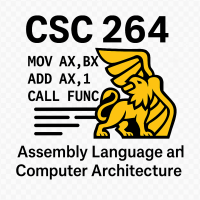
\includegraphics{../csc264Logo}
\end{center}
\end{document} 